\documentclass[12pt]{article}

\usepackage{amsmath}
\usepackage{amssymb}
\usepackage{graphicx}
\usepackage{color}
\usepackage[total={6in,8in}]{geometry}
\usepackage{amsthm}

\usepackage{enumitem}
\usepackage{centernot}

\newcommand{\N}{\mathbb{N}}
\newcommand{\Z}{\mathbb{Z}}
\newcommand{\Q}{\mathbb{Q}}
\newcommand{\R}{\mathbb{R}}
\newcommand{\C}{\mathbb{C}}
\newcommand{\sn}{\mathfrak{S}}
\newcommand{\ve}{\varepsilon}
\setlength{\parindent}{1cm}


\author{Marika Swanberg and Jillian James}
\title{Cache Optimization}
\date{}
\begin{document}
\maketitle
\section{Optimization}
Our data from last homework showed a sharp increase in the average response time as we increased the number of items in the cache. We hypothesized that this was due to how our FIFO eviction was implemented. Initially, we implemented FIFO by associating every element in the \texttt{unordered\_map} implementation of our cache with an 'age' value. Then when we evicted we would search through the map for the 'oldest' value and delete it. This made our eviction algorithm essentially $O(n)$. For very large caches, this eviction method is very bad. We decided that this would be the most important thing to optimize, so we focused our energy here. 

We decided to replace this method with a simple queue. In order to do this, we made changes to our \texttt{unordered\_map} implementation, the eviction method, the set function, and the get function. Where we used to store 3-tuples in our \texttt{unordered\_map}, we now store 2-tuples since we no longer keep track of the ages of cache elements. Our \texttt{set()} method enqueues items and our \texttt{evictor()} method dequeues the item and deletes that item from the cache. This is an $O(1)$ algorithm that we overlooked while writing our initial implementation.


\section{Benchmarking}
The homework 6 description says to "assume a fixed workload mix of $70\%$ GETs, $30\%$ SETs, and a $90\%$ hit ratio for GET requests; in addition, we'll set all key sizes arbitrarily at 8 bytes and values sizes at 16 bytes (this is not entirely representative, but will allow uniform comparison between different projects". This standard wouldn't work well for us. In Homework 5 we made a workload that was supposed to mimic that of Memcached. The Memcached paper presented a GET:SET ratio of 30:1 so to best simmulate this on homework 5, we had a workload of around $95\%$ GETS, $4\%$ SETS, and $1\%$ DELETES (These deletes are the ones called by the host using the DEL method, not the ones that happen as a result of eviction as those occur very frequently for small cache sizes). Additionally, because our network and host use keys and values that are strings, the key and value sizes are the size of std::string. Therefore, in order to get the best measurements on how much our cache improved, we used the same workloads and standards used in homework 5.

\section{Results}
\bigskip 

\begin{figure}
\centering
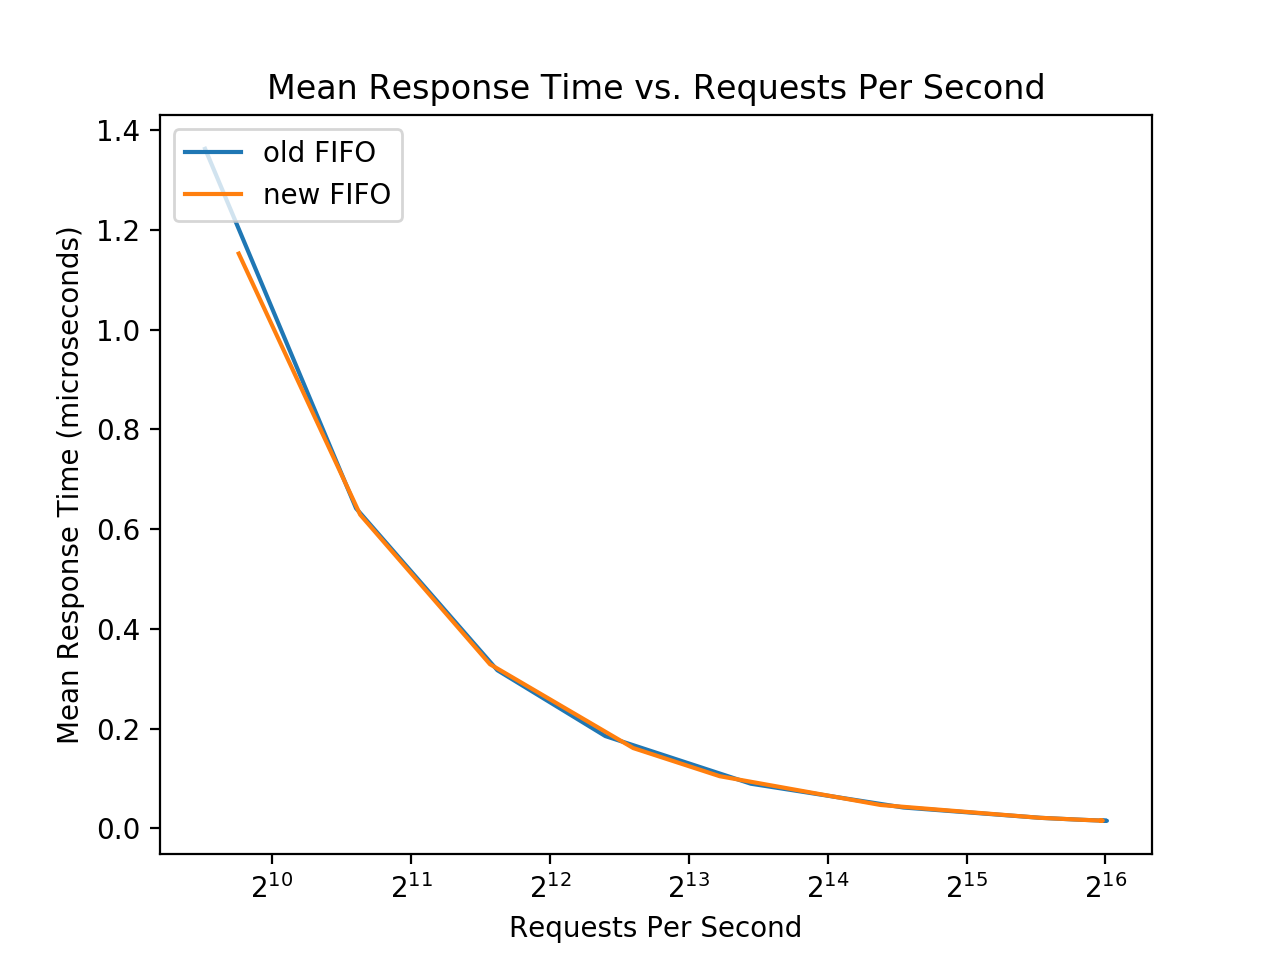
\includegraphics[scale=0.75]{reqs_per_sec_newold.png}
\caption{Mean response time as requests per second increase. We used the workload described, 95\% GETS, 4\% SETS, and 1\% DELETES. The cache was initialized with 10000 items in the cache before benchmarking the response time. Note that the old and new implementations of FIFO perform the same on average. This is to be expected because the workload that we selected for homework 5 does not exercise the evictor, so our average case is about the same on this workload.}
\end{figure}


\begin{figure}
\centering
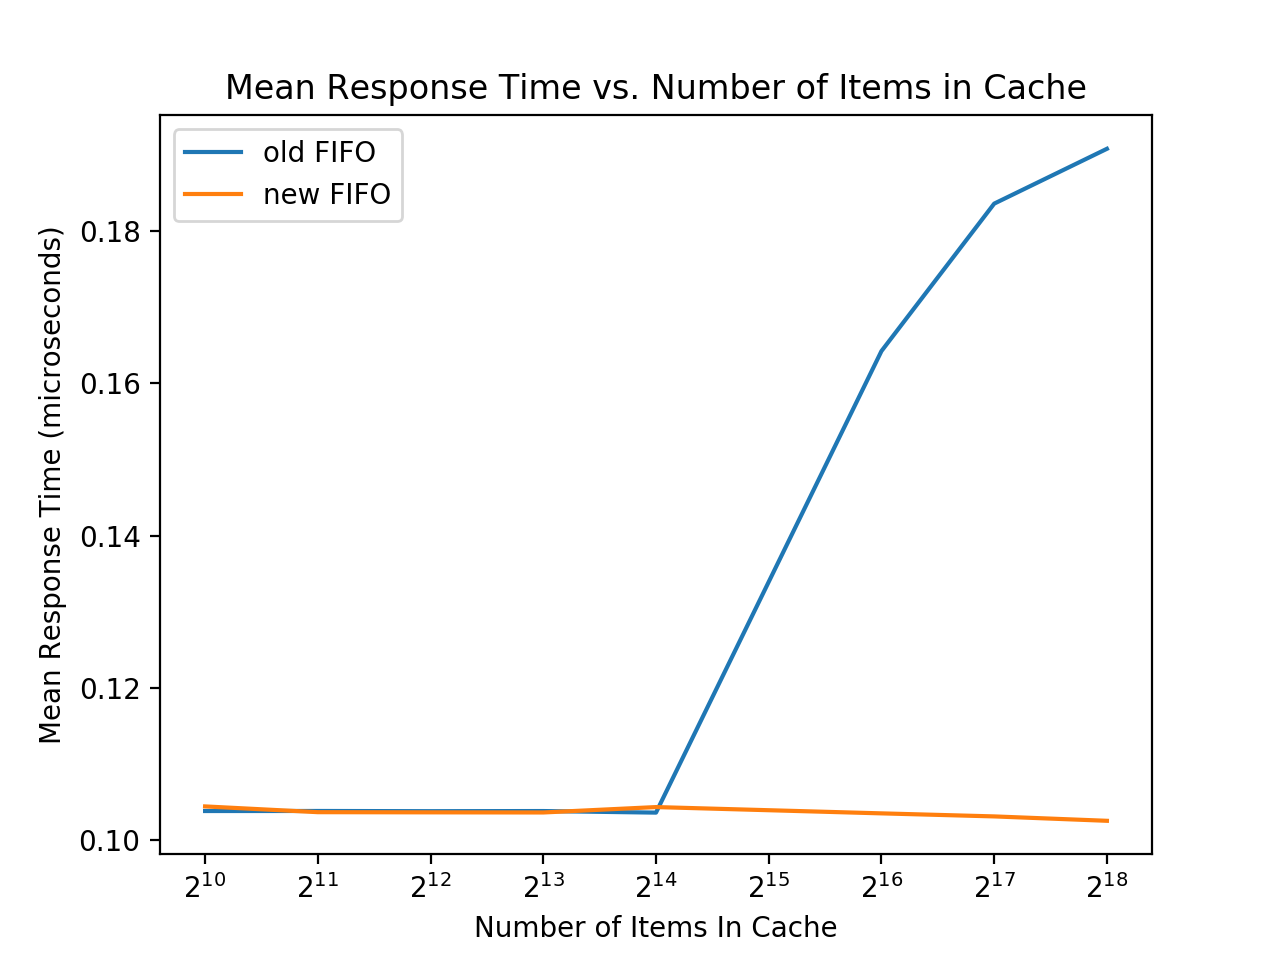
\includegraphics[scale=0.75]{resp_time_items_cache_newold.png}
\caption{This figure illustrates the response time as a function of how many items (of equal size) are in the cache. We initialized the server cache with $60,000 \approx 2^{16}$ bytes for the  benchmark, and simply increased the number of items that we tried to cram into the cache. We kept the requests per second constant at 10,000, which is why 0.1 microseconds is the lowest response time. The sharp increase in response time for the old FIFO implementation at $2^{14}$ is when the eviction policy was used during SET operations (only 4\% of the total workload).}
\end{figure}

We were able to significantly decrease the response time for our SET operation, which was $4\%$ of the workload, by improving the implementation of FIFO (see Figure 2). The average response time did not change when the eviction policy was not being exercised (Figure 1), but it was a factor of $n$ faster when evictions were taking place. 

The old FIFO implementation showed a sharp increase in the response time at around $2^{14}$ items in the cache, which is $2^{14} \cdot 32 = 2^{19}$ bytes because the values in the cache were all strings of 32 bytes each. We initialized the cache with $60,000 \approx 2^16$ bytes, so we would expect the cache to fill up after $2^{11}$ items were in the cache. It is unclear why exactly the evictions began happening at $2^{14}$, but improving our FIFO implementation gave us a substantial performance improvement. 
